\documentclass[main.tex]{subfiles}
\begin{document}
\begin{flushright}
	\begin{kaishu}
		感人的歌声留给人的记忆是长远的。\\
	\end{kaishu}
	- 摘自中学语文课文
\end{flushright}

\begin{figure}[h]
\centering
\begin{minipage}{.45\textwidth}
	\centering
	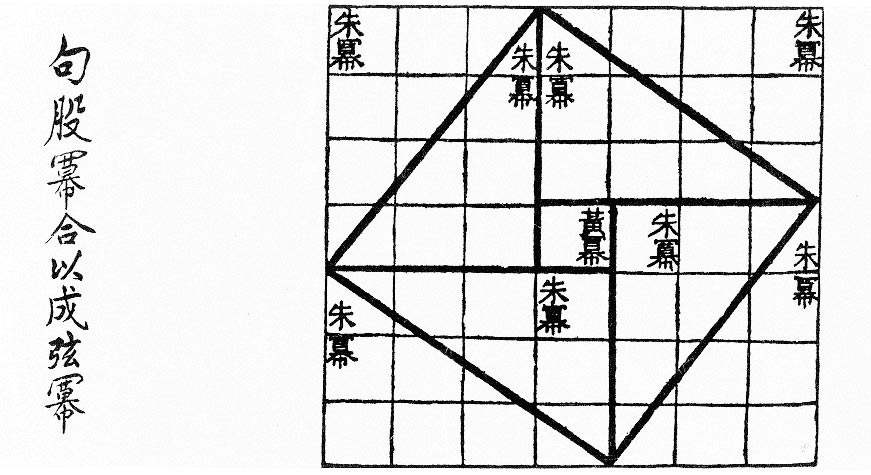
\includegraphics[width=0.8\textwidth]{jpg/gougu.jpg}
	%	\label{fig:1.5.2}
\end{minipage}
\begin{minipage}{.45\textwidth}
	\centering
	
\includegraphics[width=0.44\textwidth]{eps/gougu.eps}
%    \label{fig:chap1.5.1}
\end{minipage}
\caption{勾股定理}
 \label{fig:1.5.1}
\end{figure}	

{《周髀算经》勾股定理图}

勾股定理 - 北京2002年国际数学家大会会标中的图案
\begin{figure}[h]
	\centering
	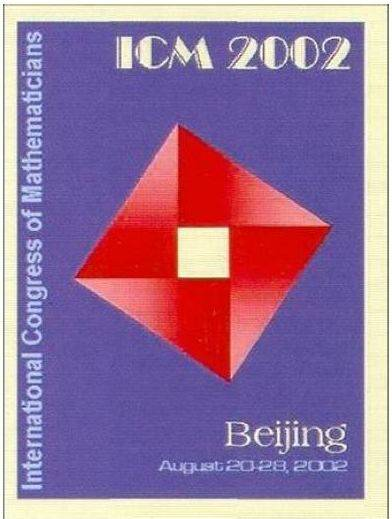
\includegraphics[width=0.5\textwidth]{jpg/icm2002.jpeg}
	\caption{北京2002年国际数学家大会会徽}
	\label{fig:chap1.5.3}
\end{figure}	

对每个正整数$n$,在抛物线$y=x^2$的杯子中间作半径为$n$的圆与之相切.则根据中学的解析几何进行计算,切点为$(\sqrt{n^2-1/4}, \pm(n^2-1/4))$,圆心为$(0,n^2+1/4)$.各圆也正好相切.
于是,在旋转拋物面$z=x^2+y^2$中从公元元年开始,每个新的公元$n$年可放入一个半径为$n$的球体,使它们完美地与曲面互切并与上年的球体刚好相切.冷饭可以年年热炒恭贺新年.

\end{document} 
